\section{Methodology}
\subsection{Direct Simulation Monte Carlo method}
The Direct Simulation Monte Carlo method  was initially introduced by Graeme A. Bird in the 1960s, and has become with time the de facto standard for rarefied flow simulations. When it was first developed, this method represented a radical departure from the traditional approaches employing a mathematical description of the flow, to such an extent that many questioned the validity of its results. It was eventually proven though, that, for time step and cell size tending to zero, the DSMC method converges to a solution of the Boltzmann equation \cite{bird}.

This method models the gas as a large collection of simulated particles, each representing an even wider set of real molecules. These molecules are propagated through the simulation domain, where they collide in a stochastic manner. \cite{themontecarlo}.

As the name in itself implies, this method is statistical at heart. Its results are in fact based on averaging the microscopic quantities of each of the molecules over a high number of time steps and over the grid cell size, in order to obtain global aerodynamic quantities. \cite{bird, themontecarlo}. This process will be discussed more in depth in \autoref{subsection:sampling}

\subsubsection{Particle description}
As mentioned previously, DSMC employs a particle description of the flow. The number of simulated particles is usually significantly lower than the real number of particles in the problem. This is due to the immense computational expense that simulating all of the particles in the real domain would require \cite{natodsmc}. To provide some perspective, it is useful to consider one of the most rarefied simulations conducted as part of this thesis. In this scenario, with a Knudsen number of 10 and a density of \qty{2e-7}{\kg\per\meter^3} (a mere 0.00001\% of the air density at sea level), more than \qty{3.6e18}{} molecules per cubic meter would have been required if a one-to-one correlation between the real and simulated molecules were to be maintained. The ratio between real and simulated molecules is expressed by $f_{num}$.

At the beginning of each simulation, a reference set of simulation particles is created. The microscopic properties (position and velocity) of each of the molecules in this set are chosen such that the bulk velocity and the global temperature of the flow correspond to the ones specified by the user, and that the number of simulated particles in the domain is equal to $\frac{n_{real}}{f_{num}}$. The velocity of the particles is usually selected at random through a Maxwell-Boltzmann distribution \cite{natodsmc}.

The simulated particles are not identical to the real particles: to correctly simulate the behaviour of the system the radius of each simulated particle must be proportional to the number of real particles that it represents, and is thus calculated such that \autoref{eq:radius} is valid. This approach also ensures the correct number of collisions in the flow \cite{dsmcnotes}.
\begin{equation}
    n_{real}\, \sigma_{real} = n_{sim}\, \sigma_{sim}
    \label{eq:radius}
\end{equation}
No indication of how the mass of each of the simulated particles is determined has been found in literature. However, based on how the SPARTA DSMC code calculates surface quantities, it is the author's understanding that the mass of the simulated particles is equal to the mass of the real particles.

\subsubsection{Mesh}
The DSMC method discretises the domain into a collection of mesh elements. This might seem counter intuitive, as the method operates on a particle-based description of the flow, which does not require the solution of any partial differential equation.

The mesh discretisation serves two main purposes: 

\begin{itemize}
    \item It allows to reduce the computational expense: employing pure Newtonian mechanics for all the molecules within the simulation domain would be too computationally expensive \cite{themontecarlo}. Thus DSMC only computes collision of randomly selected molecules within the same cell, disregarding collisions between molecules belonging to different cells, significantly cutting the computational burden. This topic will be discussed in more detail in \autoref{subsection:collision}
    \item It allows the calculation of global quantities such as temperature, bulk flow velocity or density by averaging the microscopic properties of the simulated particles over the cell volume. More details about this process can be found in section \autoref{subsection:sampling}.
\end{itemize}

As an added benefit, discretising the domain allows to parallelise the code by assigning chunks of cells of each processor, thus lowering the time required for the simulation.

\subsubsection{Boundary conditions}
One of the main advantages of the DSMC method is the ease of computing and assigning boundary conditions. Generally speaking, five boundary conditions exist \cite{natodsmc, spartadoc}
\begin{itemize}
    \item Outflow boundary: particles that cross this boundary are removed from the simulation.
    \item Inflow boundary: this type of boundary acts as a reservoir with gas properties specified in the simulation file. Particles are emitted into the simulation based on a surface generator (where the number of particles to be injected is determined from the number flux and their velocity from a surface distribution) or a volume generator (where a layer of "ghost cells" is created and filled with particles that satisfy the reference state properties, and the ones that do not cross the boundary after the particle move are discarded) \cite{natodsmc}. An inflow boundary also acts as an outflow boundary for particles that cross it from the simulation domain.
    \item Periodic boundary: the particles that cross this boundary exit the simulation and re-enter it at the opposite boundary (e.g., if the top of the simulation is a periodic boundary, particles will re-enter the simulation from the bottom) with unchanged velocity.
    \item Specular boundary: particles that cross this boundary reflect off of it with inverted normal velocity.
    \item Surface/thermal wall: particle that cross a surface are scattered based on the chosen surface-particle interaction model. More details will be given in \autoref{subsection:partsurf}.
\end{itemize}

\subsubsection{Particle motion}
\label{subsection:motion}
Particles propagate through the simulation domain based on ordinary Newtonian mechanics. \autoref{eq:posupdate} shows the position update equation \cite{bird}, where $\mathbf{r}$ is the position vector of the particle, $\mathbf{v}$ is the velocity of the particle and $\Delta{t}$ is the time step.
\begin{equation}
    \Delta{\mathbf{r}} = \mathbf{v}\, \Delta{t}
    \label{eq:posupdate}
\end{equation}

\subsubsection{Particle collision selection}
\label{subsection:collision}
As previously mentioned, particle collisions are handled by DSMC with a probabilistic rather than deterministic approach. While it may seem intuitive to compute the trajectories of all the particles within a cell and check for collisions for each pair, or focus on nearby particles, DSMC takes a different approach.

In DSMC collision pairs are chosen at random, without taking into consideration their position or proximity to one another. A collision probability $P$, independent of the relative position of the molecules, is then computed, and the collision is said to happen with probability P \cite{bird, themontecarlo, natodsmc}.

The sequence of steps taken is the following:
\begin{enumerate}
    \item The number of candidate particles is computed based on \autoref{eq:candidate} \cite{themontecarlo}, where $N_{\mathrm{c}}$ is the number of particles in the cell, $\sigma$ is the collisional radius of the simulated molecules, $v_{\mathrm{r}, \max }$ is the maximum relative velocity and $V_{\mathrm{c}}$ is the cell volume.
    \begin{equation}
        N_{\mathrm{cand}}=\frac{N_{\mathrm{c}}^2\, \pi\, \sigma^2\, v_{\mathrm{r}, \max }\, f_{num}\, \Delta t}{2 V_{\mathrm{c}}}
        \label{eq:candidate}
    \end{equation}
    \item A pair of potential collision partners is randomly selected among the particles in the cell, and their collisional probability $P$ is computed. The collisional probability formula varies based on the chosen interaction model \cite{natodsmc}, but is usually proportional to both the collisional radius of the molecules and their relative velocity \cite{bird}.
    \item The pair is accepted as collision partners if their collision probability is higher than a random variable sampled from a uniform deviate in (0, 1) \cite{themontecarlo}.
    \item If the pair is accepted as collision partners, the new velocities of the molecules are computed and the algorithm moves to the next pair. Otherwise the algorithm moves to the next pair without modifying the velocities.
    \item The algorithm is repeated until the number of candidate particles is reached.
\end{enumerate}

\subsubsection{Intermolecular collision mechanics and models}
When particle collide with each other, their velocities are computed based on the chosen intermolecular collision model. All of the intermolecular collision models encountered in literature are partly based on momentum conservation, as in \autoref{eq:momcons}. The extra equations are derived based on the specific collision model
\begin{equation}
    m_{1,i}\; v_{1,i} + m_{2,i}\; v_{2,i} = m_{1,f}\; v_{1,f} + m_{2,f}\; v_{2,f}
    \label{eq:momcons}
\end{equation}
The three most commonly employed models are:
\begin{itemize}
    \item Hard sphere model: this model treats molecules as impenetrable hard spheres with fixed collision diameter. Velocities are computed based on elastic collision theory \cite{collisionmodels}.
    \item Variable hard sphere (VHS) model: this model is based on the hard sphere model, but it expands it by considering a variable collision diameter, based on the particle relative velocity. Post collision velocities are again determined based on elastic collision theory. This method resulted in scattering which was in poor agreement with the experimental results, which led to the development of the variable soft sphere model \cite{collisionmodels}.
    \item Variable soft sphere (VSS) model: this model introduces an extra parameter $\alpha$, which governs the post collision scattering of the particles (which becomes anisotropic) \cite{collisionmodels}.
\end{itemize}

Many more models exist, such as the Generalized Hard Sphere (GHS) or Lennard-Jones (L-J) models \cite{collisionmodels}, but they are beyond the scope of this dissertation.

\subsubsection{Particle-surface interactions}
\label{subsection:partsurf}
As for particle-particle interactions, many models exist for particle-surface interaction. The two most commonly used ones are:
\begin{itemize}
    \item Specular reflection: this model reflects the particle with inverted normal velocity and unchanged parallel velocity. Since there is no change in velocity, no energy is transferred to the surface.
    \item Diffuse reflection: this model reflects the particles independently of their velocity before reflection. The post collision velocity is usually determined from a Maxwellian distribution based on the wall temperature \cite{bird, spartadoc}.
\end{itemize}

Many solvers allow to employ both the models at the same time through an accommodation coefficient, which determines what fraction of the collisions will be of each type.

More information about more advanced models can be found in \cite{spartadoc}.

\subsubsection{Sampling and calculation of global quantities}
\label{subsection:sampling}

To obtain useful global quantities from the microscopic properties of the molecules, a particle sampling is executed. This consists in determining the gas macroparameters by aggregating the molecular quantities of simulated particles and averaging them over the cell volume. 

\autoref{eq:density}, \autoref{eq:velocity}, and \autoref{eq:ke} respectively outline the mathematical process employed to execute the sampling for density, mass-weighted average u velocity, and average kinetic energy in the SPARTA DSMC code. In the aforementioned equations $f_{num}$ is the real to simulated particles ratio, $V_{\mathrm{c}}$ is the cell volume, $N_{\mathrm{c}}$ is the number of particles in the cell, $m_i$ is the mass of each particle and $u_i$, $v_i$, $w_i$, are respectively the $x$, $y$ and $z$ components of velocity.
\begin{equation}
    \rho = \frac{f_{num}}{V_{\mathrm{c}}}\; \sum_{i=1}^{N_{\mathrm{c}}}\; m_i
    \label{eq:density}
\end{equation}
\begin{equation}
    u = \frac{\sum_{i=1}^{N_{\mathrm{c}}}\; u_i\; m_i}{\sum_{i=1}^{N_{\mathrm{c}}}\; m_i} 
    \label{eq:velocity}
\end{equation}
\begin{equation}
    KE = \frac{1}{N_c}\; \sum_{i=1}^{N_{\mathrm{c}}}\; \frac{1}{2}\; m_i\; (u_i^2+v_i^2+w_i^2)
    \label{eq:ke}
\end{equation}
A similar procedure can be employed to get surface-specific values, such as the heat transfer or the force applied to a surface element.

Given the statistical noise inherent of a Monte Carlo method, the macroscopic quantities are also usually averaged over a number of time steps.

\subsubsection{Iterative procedure}
When a Direct Simulation Monte Carlo code is run, the following procedure is executed:
\begin{enumerate}
    \item A random seed for the simulation is set. This set will be used to randomly generate the set of initial particles and the particles emitted by the inflow boundaries.
    \item The simulation domain is created,the mesh and the reference set of initial particles are generated, and the internal geometry is loaded.
    \item The number of iterations $n$ and the initial time $t$ are set to zero.
    \item The particles are propagated through the simulation domain as described in \autoref{subsection:motion}.
    \item Collisions between particles and boundaries/surfaces is checked. New velocities of the particles are computed and assigned. Particles are inserted or removed into the domain.
    \item Particles are indexed, meaning their position is used to determine to which cell they belong to, to subsequently compute inter-particle collisions.
    \item Inter-particle collisions are computed and new velocities assigned.
    \item $n$ is incremented by 1, $t$ by $\Delta t$.
    \item If the simulation has reached steady state, the particle sampling is executed as described in \autoref{subsection:sampling}, otherwise the loop continues.
    \item If the final time has been reached, the results are printed and the simulation is stopped, otherwise the process goes back to step 4.
\end{enumerate}

\autoref{fig:dsmcflowchart} shows the steps outlined above in a flowchart.

\begin{figure}[ht]
    \centering
    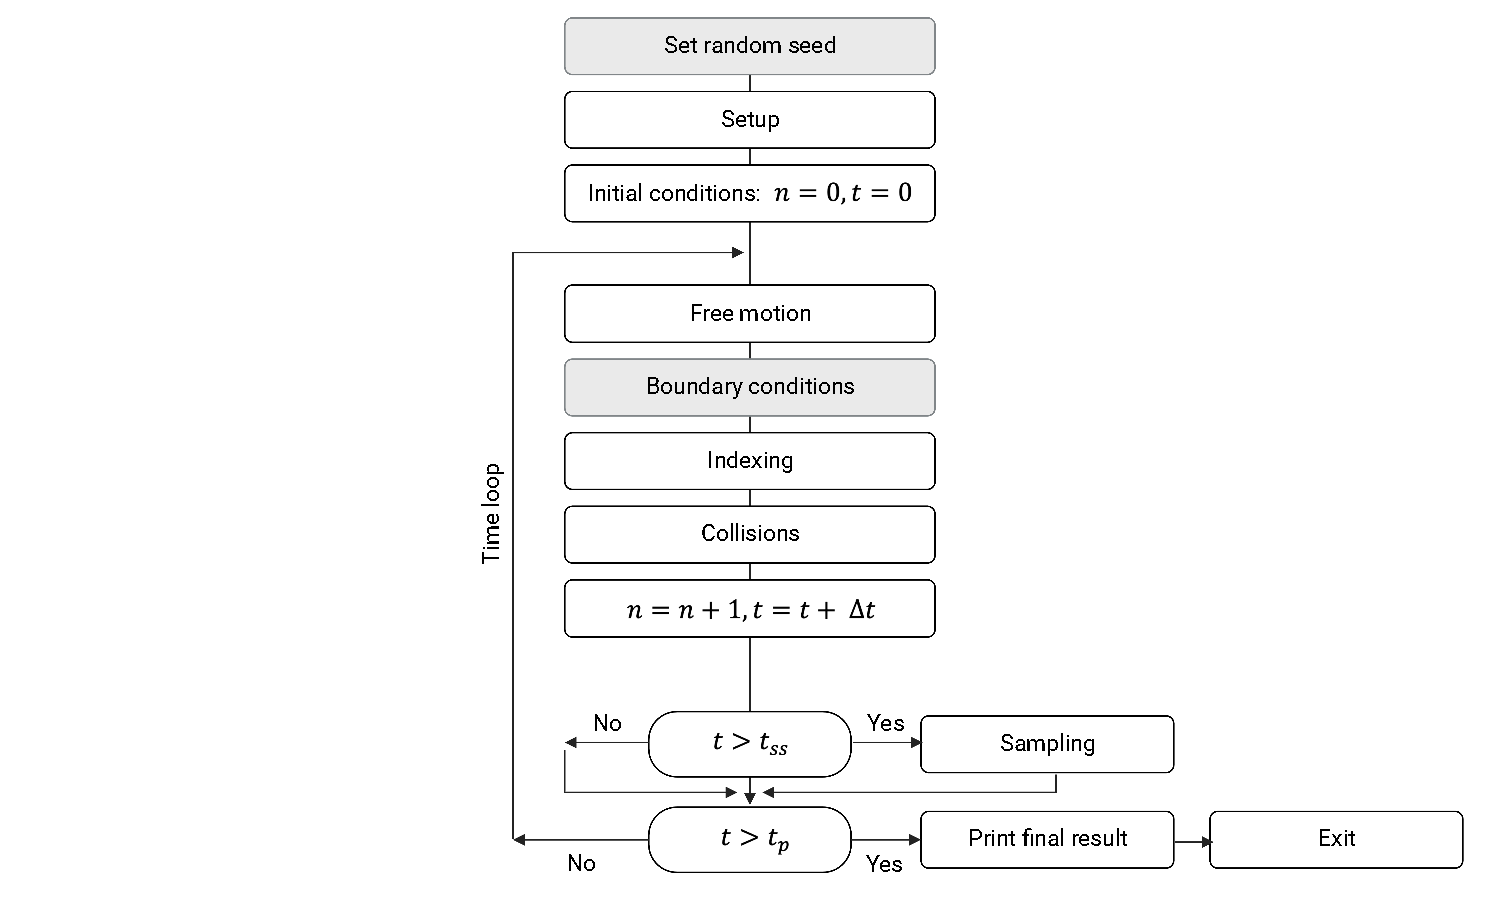
\includegraphics[width=\textwidth]{../Images/3. Methodology/dsmcflowchart.pdf}
    \caption{Flowchart of DSMC method loop. Adapted from \cite{dsmcnotes}.}
    \label{fig:dsmcflowchart}
\end{figure}

\subsubsection{DSMC best practices}
\label{subsection:bestpractices}
Literature indicates some general good practices for running DSMC algorithms. Three main parameters have to be taken into consideration for the successful execution of a simulation \cite{purdue}: the mesh size, which has to be kept below one third of the mean free path \cite{purdue, fnum1}, the time step, which has to be kept below one third of the smaller between the mean collision time and the mean transition time \cite{purdue}, and the number of simulated particles, which has to be kept to around 20 per cell \cite{purdue}. 

It has to be pointed out that the latter requirement has been proven significantly less relevant than the former two \cite{fnum1, fnum2}. However, this requirement will still be applied in the simulations, for reasons discussed in \autoref{subsection:fnum}.

\subsection{Choice of software package}
Three pieces of software were considered for running the simulations: dsmcFoam, a Direct Simulation Monte Carlo implementation part of the more general OpenFoam CFD package \cite{openfoam}, its expansion from the rarefied hypersonics team at Strathclyde university dsmcFoam+ \cite{dsmcfoam+}, and the SPARTA DSMC code from Sandia National Laboratories \cite{sparta}.

dsmcFoam was employed for several weeks and numerous test simulations were run on it. However, a decision was made to replace it, primarily due to its intricate operation and the lack of readily available documentation or a supportive user community. It was initially decided to replace it with dsmcFoam+, but some incompatibilities with the departmental HPC server prevented its use. The SPARTA DSMC package was thus chosen.

\subsection{Simulation design}
The simulations were designed around simple shapes, that presented the generic features  and flow structure of the aeroshells in \cite{hathoraero1} while ignoring irrelevant details such as the nose radius or the cone half angle. The geometries also had to highlight the local rarefaction effects with respect to the global flow. The best geometry for this purpose was deemed to be a square with rounded corners, since it presented two edges, representative of the tip of the aeroshell, and a significant wake at the back. The rounded corner was employed to have an extra parameter to control local Knudsen number through. During the course of the research it was deemed useful to show how the flow features changed when taking the corner radius to extremes. The geometries of a circle (which corresponds to the radius being equal to the side of the square) and a perfect squares (radius of zero) were also simulated.

Four sets of simulations were run: constant edge radius with varying global Knudsen number, constant knudsen number with varying edge radius, constant local Knudsen number (both edge radius and global Knudsen number vary to achieve a constant Knudsen number at the edge), varying angle of attack.

\subsubsection{Common parameters}
Before designing the individual sets of simulations, certain parameters, applicable universally across all simulations, were determined:
\begin{itemize}
    \item Mach number, which was set to 5 to replicate the one seen in \cite{rees}.
    \item Cube size, which as the mach number was set to \qty{3}{\cm} to replicate \cite{rees}.
    \item Simulation domain size, initially set to a square with side of \qty{0.2}{\m}, then increased to \qty{0.3}{\m} to encase the entire bow shock around the cube.
    \item Molecular mixture, chosen to be 22.3\% of $O_{2}$ and 77.7\% of $N_{2}$ by molecule count, to accurately represent the standard composition of air.
    \item Mixture temperature, chosen to be \qty{273}{\kelvin}.
    \item Surface collision accommodation parameter, set to 0.85 in accordance with \cite{accomod}
    \item Surface temperature of the geometry set to \qty{300}{\kelvin}.
\end{itemize}

Some of these parameters, such as the geometry and mixture temperature, along with others that will be mentioned subsequently, were selected arbitrarily as they did not directly influence the simulation outcomes. Their values were primarily used to generate the targeted non-dimensional numbers. For instance, to achieve a specific Reynolds number, parameters like viscosity, velocity, and size were arbitrarily fixed, and then the density was computed accordingly.

All of the simulations were run as 2D simulations, 

Two more parameters were needed to fully characterise the simulation: number density and real to simulated particles ratio. Their derivation will be explored in the following section.

\subsubsection{Varying Knudsen number}
For the varying Knudsen number case, it was initially planned to run a set of simulations which spanned the slip flow regime (between Knudsen numbers of 0.01 and 10). For completeness of results, two more simulations were added towards the end of the project, at Knudsen numbers of 0.001 and 100.  The chosen values can be seen in \autoref{tab:kn}. 
To compute the number density for each of the test cases, the following procedure was used:
\begin{enumerate}
    \item Determined Reynolds numbers as $\frac{M}{Kn}$.
    \item Calculated flow velocity from $M = \frac{u}{a}$ with $a = \sqrt{\gamma R T}$.
    \item Calculated flow viscosity from Sutherland's law.
    \item Calculated density from $Re = \frac{\rho\, u\, d}{\mu}$.
    \item Calculated the average molecule mass by computing the weighted average of the masses of $O_{2}$ and $N_{2}$, as in \autoref{eq:waverage}.
    \item Calculated the required number density by dividing the density by the average molecule mass.
\end{enumerate}
\begin{equation}
    m_{mean} = 0.223\; m_{O_{2}} + 0.777\; m_{N_{2}}
    \label{eq:waverage}
\end{equation}
Having determined the number density, the ratio between real and simulated particles had to be computed. To do this, the number of real particles in the simulation domain was calculated by multiplying the density ratio by the domain volume. This value was then divided by the total number of simulated particles in the domain (computed as the product between number of cells and simulated particles per cell). The results of this calculation are shown in \autoref{tab:kn}. The process through which  the number of molecules per cell and the number of cells was determined will be discussed in a following section.

\begin{table}[h]
    \centering
    \caption{Varying Knudsen number simulations flow properties}
    \begin{tabular}{c|cccc}
        \toprule
        Simulation & Knudsen Number & Density (\si{\kg\per\m^3}) & Number density & Particle ratio\\
        \midrule
        1 & 0.001 & \num{1.727e-3} & \num{3.60e22} & \num{3.24e13}\\
        2 & 0.01 & \num{1.727e-4} & \num{3.60e21} & \num{3.24e12}\\
        3 & 0.05 & \num{3.454e-5} & \num{7.20e20} & \num{6.48e11}\\
        4 & 0.1 & \num{1.727e-5} & \num{3.60e20} & \num{3.24e11}\\
        5 & 0.5 & \num{3.454e-6} & \num{7.20e19} & \num{6.48e10}\\
        6 & 1 & \num{1.727e-6} & \num{3.60e19} & \num{3.24e10}\\
        7 & 5 & \num{3.454e-7} & \num{7.20e18} & \num{6.48e9}\\
        8 & 10 & \num{1.727e-7} & \num{3.60e18} & \num{3.24e9}\\
        9 & 100 & \num{1.727e-8} & \num{3.60e17} & \num{3.24e8}\\
        \bottomrule
    \end{tabular}
    \label{tab:kn}
\end{table}

The varying $Kn$ simulations were run for both the circle and rounded square geometries. The square edge radius was set to \qty{1e-4}{\m}. This value was chosen as .

\subsubsection{Varying edge radius}

Two sets of simulations were run for the varying edge radius case. The first set employed a Knudsen Number of 0.01 with the objective of illustrating the variation in flow structure as the edge radius increased from zero (representing a perfect square) to the length of the square side (forming a circle)
The second set of simulations was run with a $Kn$ of 0.001 and was aimed at investigating the effect of the edge radius in the change in Stanton number at the edge. The full details of the simulations can be seen respectively in \autoref{tab:radius1} and \autoref{tab:radius2}.

\subsubsection{Varying angle of attack}
The varying angle of attack simulations were conducted to investigate the variation in heat transfer at the front and back of the cube with angle of attack, as this was investigated quite extensively in literature \cite{pallahrini, spartavalid}. The simulations were run at $\pm 5$, $\pm 10$, $\pm 30$ and \qty{45}{\deg} at a Knudsen number of 0.01.
\begin{table}[ht]
    \centering
    \caption{Parameters of first set of varying edge radius simulations.}
    \begin{tabular}{c|cc}
        \toprule
        Simulation & Knudsen Number & Edge radius (\si{\m})\\
        \midrule
        1 & 0.01 & \num{0}\\
        2 & 0.01 & \num{1e-4}\\
        3 & 0.01 & \num{2e-4}\\
        4 & 0.01 & \num{5e-4}\\
        5 & 0.01 & \num{1e-3}\\
        6 & 0.01 & \num{2e-3}\\
        7 & 0.01 & \num{5e-3}\\
        8 & 0.01 & \num{1.5e-2}\\
        \bottomrule
    \end{tabular}
    \label{tab:radius1}
\end{table}
\begin{table}[ht]
    \centering
    \caption{Parameters of second set of varying edge radius simulations.}
    \begin{tabular}{c|cc}
        \toprule
        Simulation & Knudsen Number & Edge radius (\si{\m})\\
        \midrule
        1 & 0.001 & \num{0}\\
        2 & 0.001 & \num{2e-6}\\
        3 & 0.001 & \num{5e-6}\\
        4 & 0.001 & \num{1e-5}\\
        5 & 0.001 & \num{2e-5}\\
        6 & 0.001 & \num{5e-5}\\
        7 & 0.001 & \num{1e-4}\\
        8 & 0.001 & \num{1e-4}\\
        9 & 0.001 & \num{2e-4}\\
        10 & 0.001 & \num{5e-4}\\
        11 & 0.001 & \num{1e-3}\\
        \bottomrule
    \end{tabular}
    \label{tab:radius2}
\end{table}

\subsubsection{Constant local Knudsen number}
The constant local Knudsen number simulation were run while attempting to keep the local Knudsen number at the corner of the cube constant. To achieve this, a base $Kn$ and edge radius were set for the first simulation. For subsequent simulations, the Knudsen number was multiplied by a specific factor, while the edge radius was divided by the +same factor. This was done with the assumption that the local mean free path number would be directly proportional to the local one. The full set of parameters can be seen in \autoref{tab:local}
\begin{table}[ht]
    \centering
    \caption{Properties of constant local Knudsen number simulations.}
    \begin{tabular}{c|cc}
        \toprule
        Simulation & Knudsen Number & Edge radius (\si{\m})\\
        \midrule
        1 & 0.01 & \num{1e-3}\\
        2 & 0.05 & \num{2e-4}\\
        3 & 0.1 & \num{1e-4}\\
        4 & 0.5 & \num{2e-5}\\
        5 & 1 & \num{1e-5}\\
        6 & 5 & \num{2e-6}\\
        7 & 10 & \num{1e-6}\\
        \bottomrule
    \end{tabular}
    \label{tab:local}
\end{table}

\subsection{Convergence studies and validation of results}
Having designed the simulations, a set of convergence studies was run to investigate the effect of cell size, number of simulated particles and sampling time, and to determine the necessary time for the simulation itself to converge.

\subsubsection{Mesh convergence study}
To determine the optimal mesh size, a set of 8 simulations was run at a Knudsen number of 0.01. All of the simulations were run with a rounded cube with edge radius of \qty{1e-4}{\m} In the first seven simulations the number of mesh elements was manually increased from 100 to 3000 per domain dimension. The last simulation was run with a dynamically refining mesh, which started from 1000 mesh elements per dimension and dynamically split the cells containing more than 80 particles into four. The simulations were run for a total time of \qty{6e-4}{\s} and the data was sampled for the last \qty{1e-4}{\s} of the simulation. The time steps were varied in order to maintain them below a third of the mean cell transition time. The full set of simulation parameters is shown in \autoref{tab:meshconv}, together with the runtime of each of the simulations.
\begin{table}[ht]
    \centering
    \caption{Properties of constant local Knudsen number simulations.}
    \begin{tabular}{c|cccc}
        \toprule
        Simulation & Number of cells per dimension & Cell size (\si{\m}) & Time step (\si{\s}) & Runtime (\si{\s})\\
        \midrule
        1 & 100 & \num{3e-3} & \num{6e-7} & 21\\
        2 & 300 & \num{1e-3} & \num{2e-7} & 1312\\
        3 & 600 & \num{5e-4} & \num{1e-7} & 1679\\
        4 & 1000 & \num{3e-4} & \num{6e-8} & 4621\\
        5 & 1500 & \num{2e-4} & \num{4e-8} & 34464\\
        6 & 2000 & \num{1.5e-4} & \num{3e-8} & 75095\\
        7 & 3000 & \num{1e-4} & \num{2e-8} & 170914\\
        Dynamic & 4825 & Not applicable & \num{6e-8} & 18997\\
        \bottomrule
    \end{tabular}
    \label{tab:meshconv}
\end{table}

\autoref{fig:meshsec} shows the distribution of heat transfer rate around the square (more information about the x coordinate can be found in \autoref{subsection:postprocessing}) for different mesh sizes. It is possible to note that as the number of elements increases, the stagnation point heat transfer rate converges to a value of about \qty{1e+4}{\watt\per\m^2}.

\begin{figure}
    \centering
    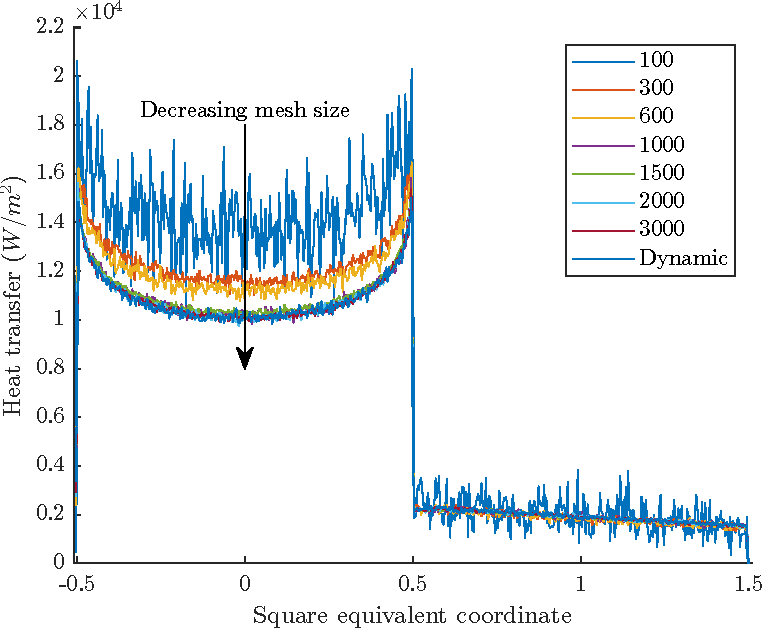
\includegraphics[width=0.7\textwidth]{Images/3. Methodology/Mesh convergence/meshsec.pdf}
    \caption{Heat transfer vs square equivalent coordinate for varying number of mesh elements.}
    \label{fig:meshsec}
\end{figure}

\autoref{fig:meshstag}, \autoref{fig:meshpeak} and \autoref{fig:meshcd} respectively show how the stagnation point heat transfer, the peak heat transfer and the drag coefficient varied when increasing the mesh resolution. In these plots the dynamic mesh was experiment was represented through a mesh size of 4825 elements, obtained by taking the square root of the total number of mesh elements at the end of the simulation.

As it is possible to see from these graphs, stagnation point heating and drag coefficient showed a lower sensibility to mesh size than peak heating, only showing respectively 1.5\% and 0.2\% of difference between the value obtained with 1000 elements and 3000 elements. Peak heating showed a slower convergence trend, only achieving full convergence past 2000 mesh elements.

Overall, all of the parameters analysed were deemed to be converged past 2000 cells per dimension. This mesh was thus validated against the best practices discussed in \autoref{subsection:bestpractices}. To do so, \autoref{eq:meanfree} was used to calculate the mean free path for the simulation with the highest density. At the time of the mesh convergence study, the planned simulation with the highest density was the one with $Kn$ equal to 0.01, with a corresponding number density of \qty{1.727e-4}{\kg\per\m^3}. This value 

\begin{equation}
    \lambda=\frac{1}{\sqrt{2} \pi \mathrm{d}^2 \mathrm{n}}
\end{equation}

and the mean collision time were calculated for the simulation with the highest density. 


This mesh size was thus selected for all of the subsequent simulations. 


\begin{figure}
    \centering
    \begin{subfigure}{0.49\textwidth}
        \centering
        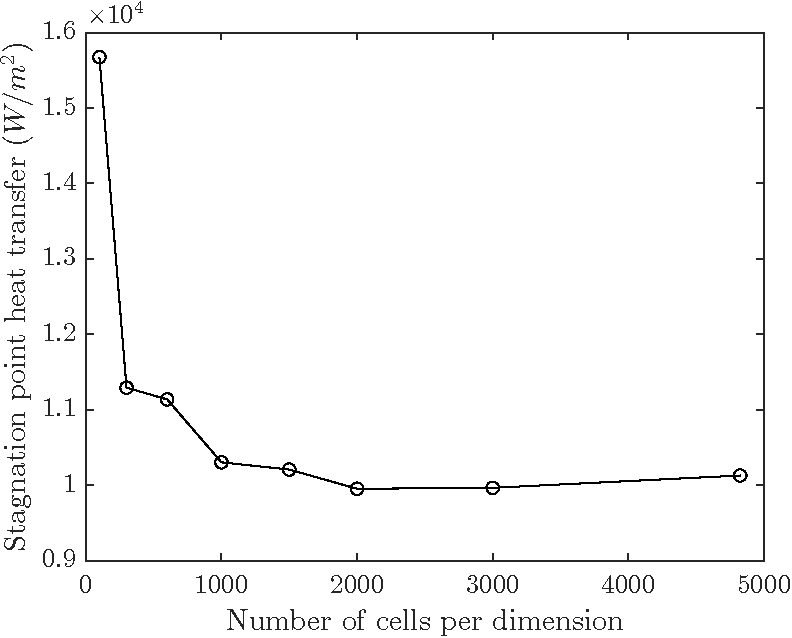
\includegraphics[width=\textwidth]{Images/3. Methodology/Mesh convergence/sphnc.pdf}
    \end{subfigure}
    \hfill
    \begin{subfigure}{0.49\textwidth}
        \centering
        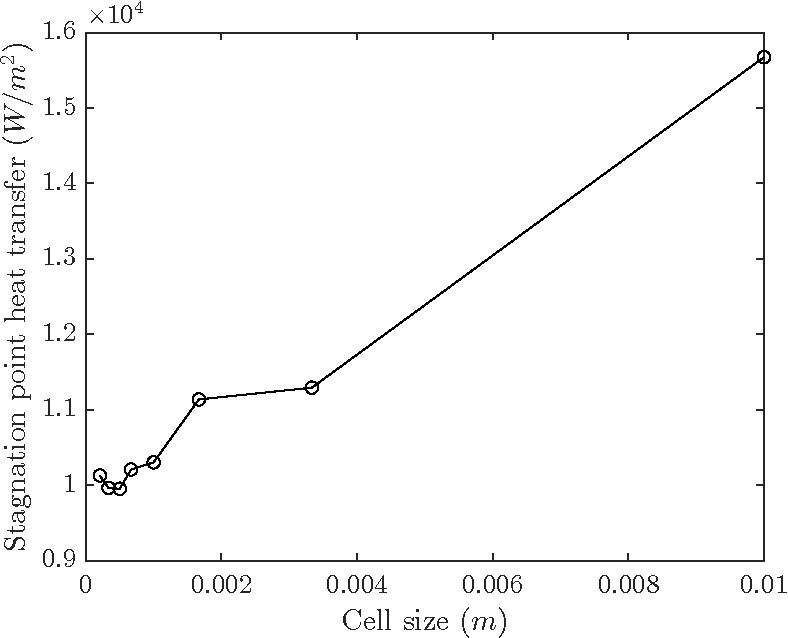
\includegraphics[width=\textwidth]{Images/3. Methodology/Mesh convergence/sphcs.pdf}
    \end{subfigure}
    \caption{Stagnation point heat transfer vs number of cells per dimension (left) and cell size (right).}
    \label{fig:meshstag}
\end{figure}

\begin{figure}
    \centering
    \begin{subfigure}{0.49\textwidth}
        \centering
        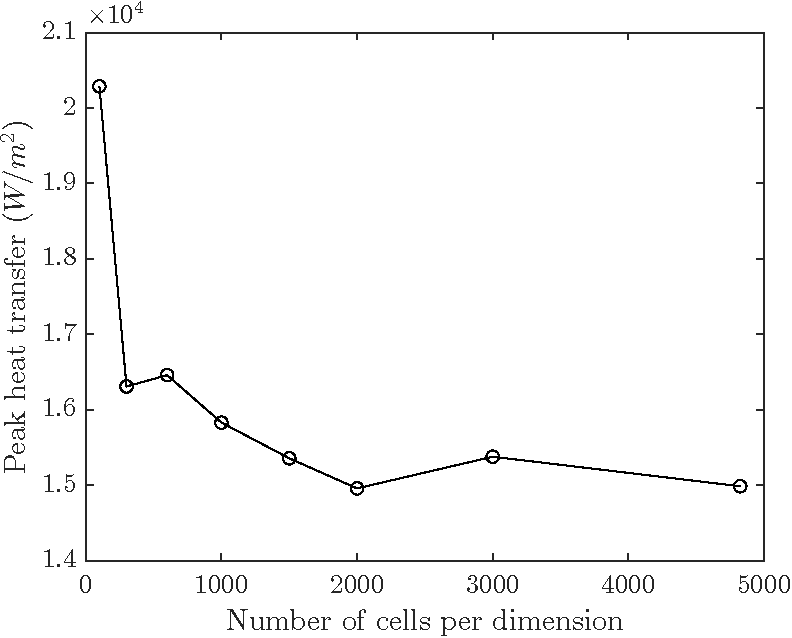
\includegraphics[width=\textwidth]{Images/3. Methodology/Mesh convergence/phnc.pdf}
    \end{subfigure}
    \hfill
    \begin{subfigure}{0.49\textwidth}
        \centering
        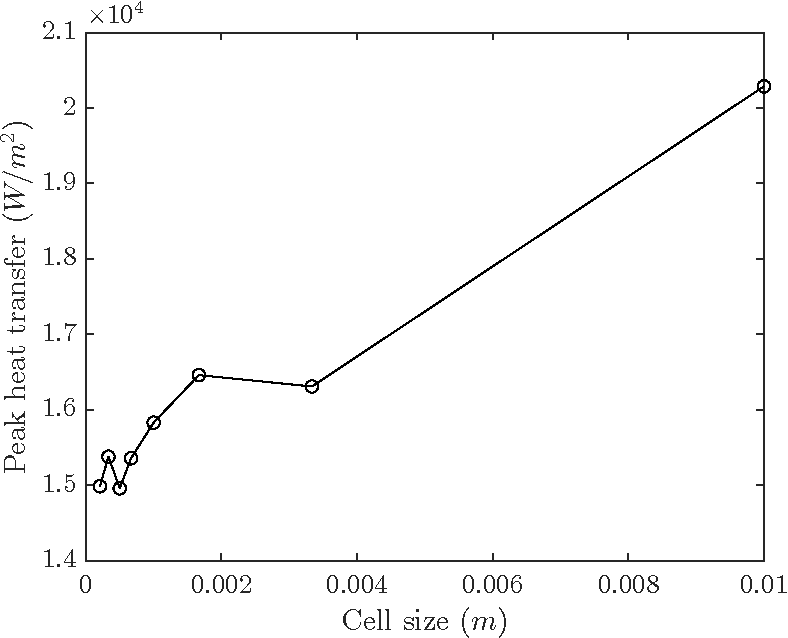
\includegraphics[width=\textwidth]{Images/3. Methodology/Mesh convergence/phcs.pdf}
    \end{subfigure}
    \caption{Peak heat transfer vs number of cells per dimension (left) and cell size (right).}
    \label{fig:meshpeak}
\end{figure}

\begin{figure}
    \centering
    \begin{subfigure}{0.49\textwidth}
        \centering
        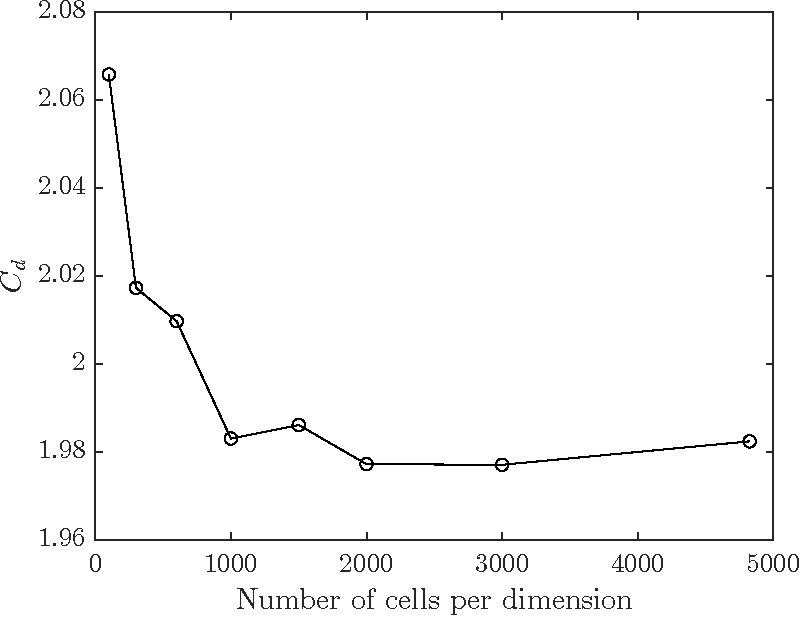
\includegraphics[width=\textwidth]{Images/3. Methodology/Mesh convergence/cdnc.pdf}
    \end{subfigure}
    \hfill
    \begin{subfigure}{0.49\textwidth}
        \centering
        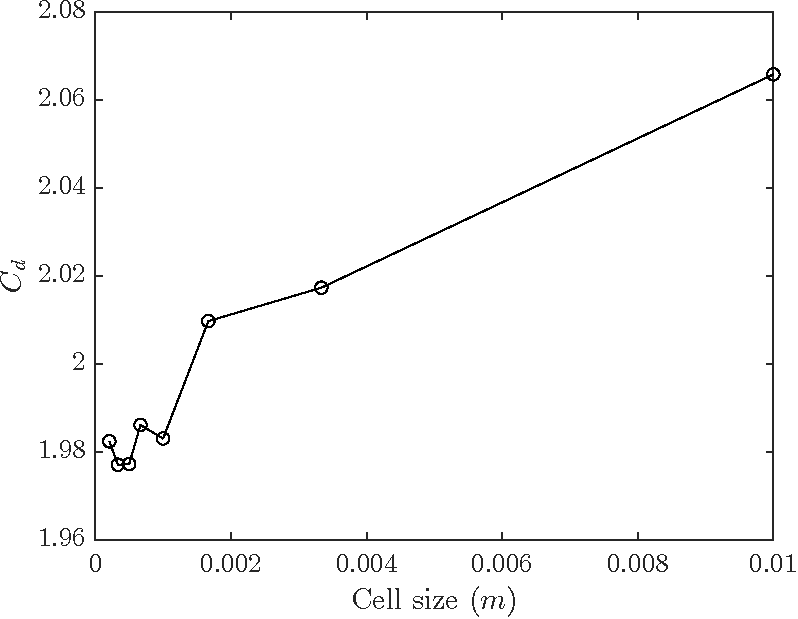
\includegraphics[width=\textwidth]{Images/3. Methodology/Mesh convergence/cdcs.pdf}
    \end{subfigure}
    \caption{Drag coefficient vs number of cells per dimension (left) and cell size (right).}
    \label{fig:meshcd}
\end{figure}

\subsubsection{Number of simulated particles convergence study}

aba

\begin{figure}[h]
    \centering
    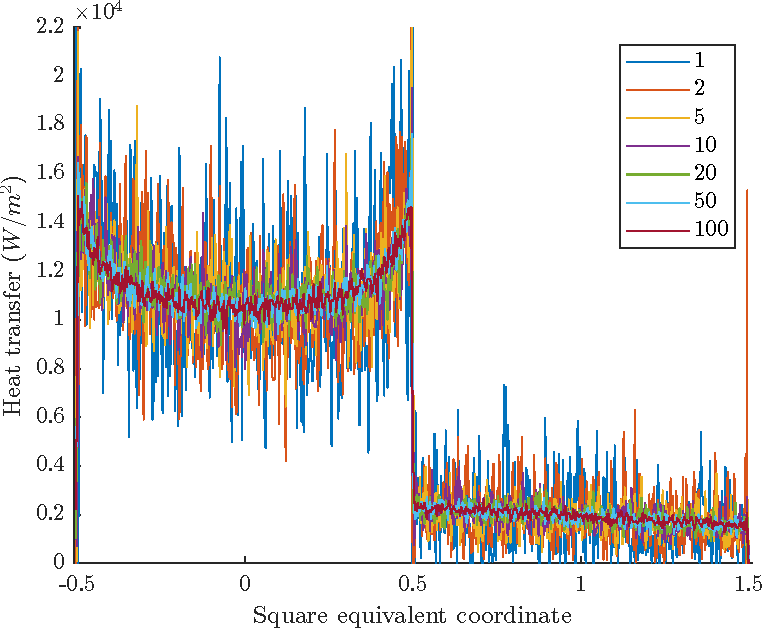
\includegraphics[width=0.7\textwidth]{Images/3. Methodology/Fnum convergence/fnumconv.pdf}
    \caption{Heat transfer vs square equivalent coordinate for varying number of particles.}
    \label{fig:fnumsec}
\end{figure}

\subsubsection{Sampling time convergence study}

\begin{figure}
    \centering
    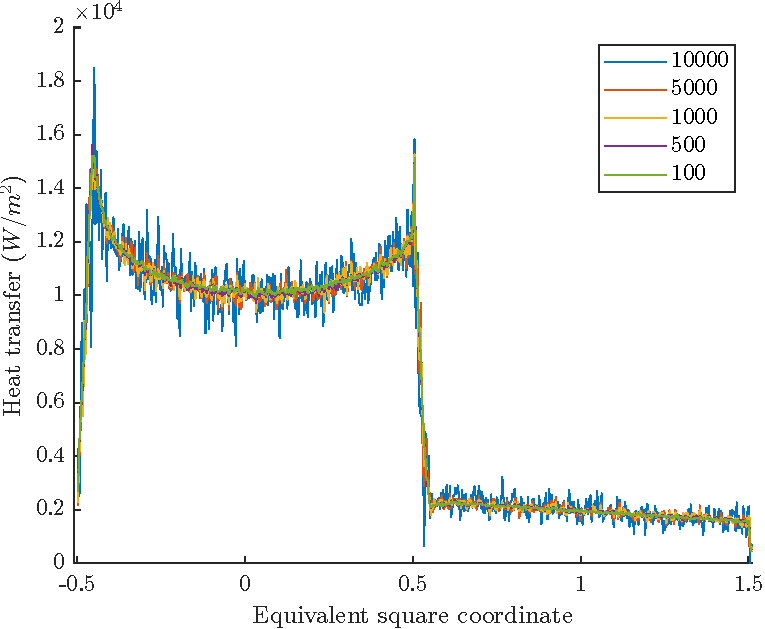
\includegraphics[width=0.7\textwidth]{Images/3. Methodology/Timestep average convergence/avesec.pdf}
    \caption{Heat transfer vs square equivalent coordinate for varying sampling time.}
    \label{fig:avesec}
\end{figure}

\begin{figure}
    \centering
    \begin{subfigure}{0.49\textwidth}
        \centering
        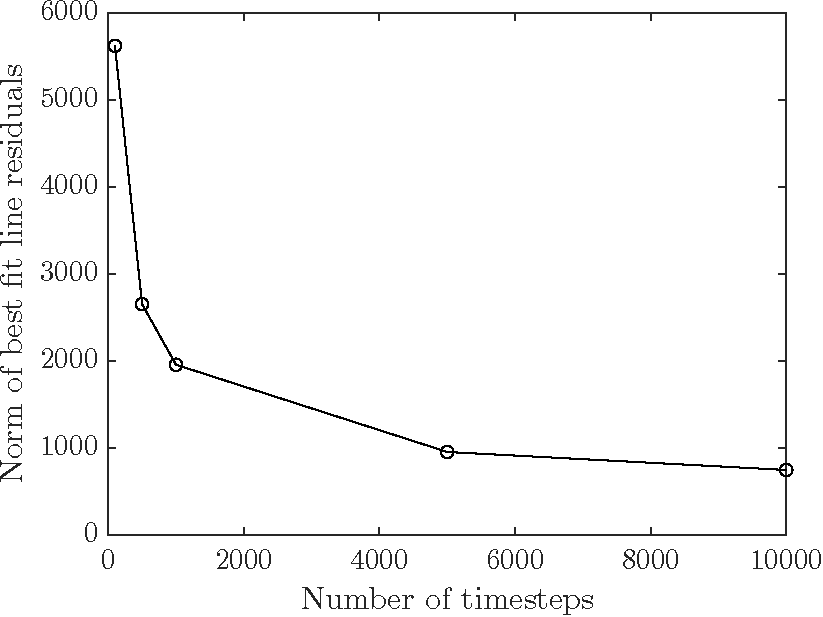
\includegraphics[width=\textwidth]{Images/3. Methodology/Timestep average convergence/rests.pdf}
    \end{subfigure}
    \hfill
    \begin{subfigure}{0.49\textwidth}
        \centering
        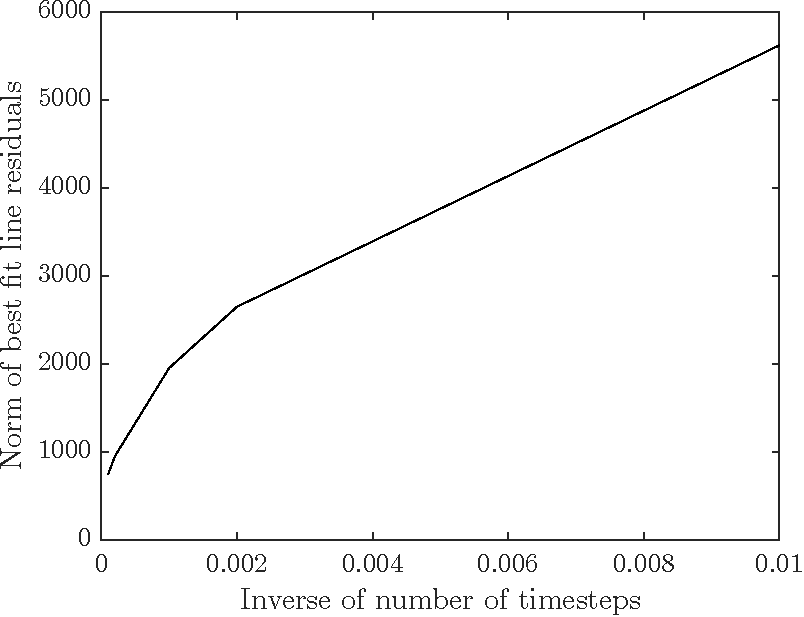
\includegraphics[width=\textwidth]{Images/3. Methodology/Timestep average convergence/resinvts.pdf}
    \end{subfigure}
    \caption{Drag coefficient vs number of cells per dimension (left) and cell size (right).}
    \label{fig:averesid}
\end{figure}

\subsubsection{Simulation convergence study}

\begin{figure}
    \centering
    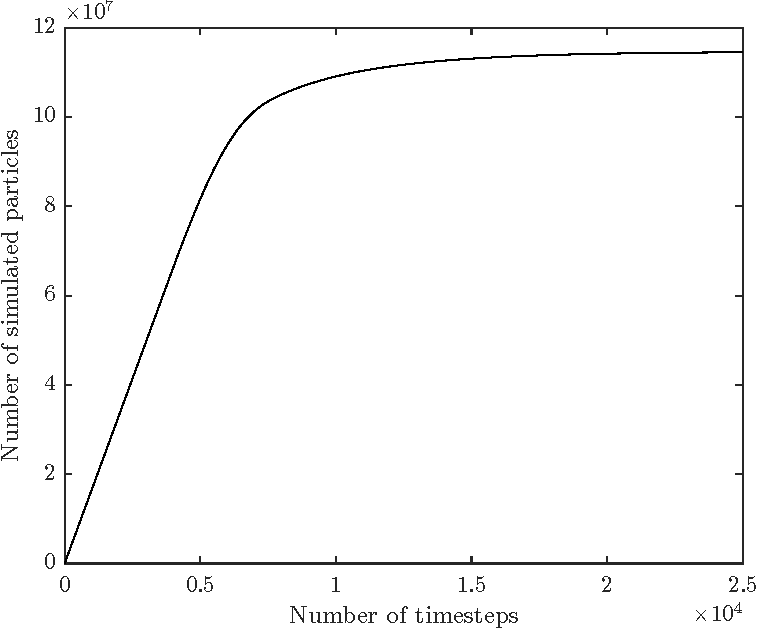
\includegraphics[width=0.7\textwidth]{Images/3. Methodology/Simulation convergence/simconv.pdf}
    \caption{Heat transfer vs square equivalent coordinate for varying sampling time.}
    \label{fig:simconv}
\end{figure}